\chapter{Mother and Son}

The Count of Monte Cristo bowed to the five young men with a melancholy
and dignified smile, and got into his carriage with Maximilian and
Emmanuel. Albert, Beauchamp, and Château-Renaud remained alone. Albert
looked at his two friends, not timidly, but in a way that appeared to
ask their opinion of what he had just done.

“Indeed, my dear friend,” said Beauchamp first, who had either the most
feeling or the least dissimulation, “allow me to congratulate you; this
is a very unhoped-for conclusion of a very disagreeable affair.”

Albert remained silent and wrapped in thought. Château-Renaud contented
himself with tapping his boot with his flexible cane.

“Are we not going?” said he, after this embarrassing silence.

“When you please,” replied Beauchamp; “allow me only to compliment M.
de Morcerf, who has given proof today of rare chivalric generosity.”

“Oh, yes,” said Château-Renaud.

“It is magnificent,” continued Beauchamp, “to be able to exercise so
much self-control!”

“Assuredly; as for me, I should have been incapable of it,” said
Château-Renaud, with most significant coolness.

“Gentlemen,” interrupted Albert, “I think you did not understand that
something very serious had passed between M. de Monte Cristo and
myself.”

“Possibly, possibly,” said Beauchamp immediately; “but every simpleton
would not be able to understand your heroism, and sooner or later you
will find yourself compelled to explain it to them more energetically
than would be convenient to your bodily health and the duration of your
life. May I give you a friendly counsel? Set out for Naples, the Hague,
or St. Petersburg—calm countries, where the point of honor is better
understood than among our hot-headed Parisians. Seek quietude and
oblivion, so that you may return peaceably to France after a few years.
Am I not right, M. de Château-Renaud?”

\begin{figure}[ht]
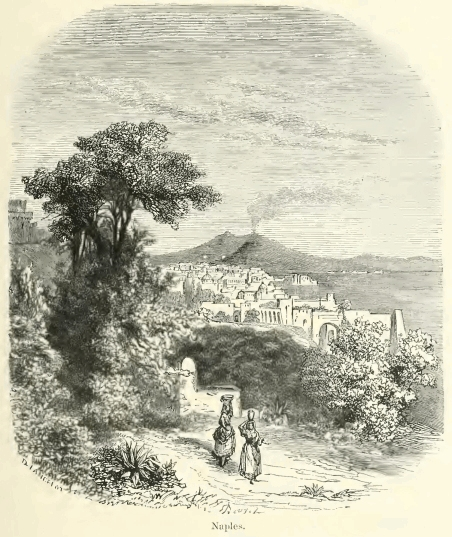
\includegraphics[width=\textwidth]{40252m.jpg}
\end{figure}

“That is quite my opinion,” said the gentleman; “nothing induces
serious duels so much as a duel forsworn.”

“Thank you, gentlemen,” replied Albert, with a smile of indifference;
“I shall follow your advice—not because you give it, but because I had
before intended to quit France. I thank you equally for the service you
have rendered me in being my seconds. It is deeply engraved on my
heart, and, after what you have just said, I remember that only.”

Château-Renaud and Beauchamp looked at each other; the impression was
the same on both of them, and the tone in which Morcerf had just
expressed his thanks was so determined that the position would have
become embarrassing for all if the conversation had continued.

“Good-bye, Albert,” said Beauchamp suddenly, carelessly extending his
hand to the young man. The latter did not appear to arouse from his
lethargy; in fact, he did not notice the offered hand.

“Good-bye,” said Château-Renaud in his turn, keeping his little cane in
his left hand, and saluting with his right.

Albert’s lips scarcely whispered “Good-bye,” but his look was more
explicit; it expressed a whole poem of restrained anger, proud disdain,
and generous indignation. He preserved his melancholy and motionless
position for some time after his two friends had regained their
carriage; then suddenly unfastening his horse from the little tree to
which his servant had tied it, he mounted and galloped off in the
direction of Paris.

In a quarter of an hour he was entering the house in the Rue du Helder.
As he alighted, he thought he saw his father’s pale face behind the
curtain of the count’s bedroom. Albert turned away his head with a
sigh, and went to his own apartments. He cast one lingering look on all
the luxuries which had rendered life so easy and so happy since his
infancy; he looked at the pictures, whose faces seemed to smile, and
the landscapes, which appeared painted in brighter colors. Then he took
away his mother’s portrait, with its oaken frame, leaving the gilt
frame from which he took it black and empty. Then he arranged all his
beautiful Turkish arms, his fine English guns, his Japanese china, his
cups mounted in silver, his artistic bronzes by Feuchères or Barye;
examined the cupboards, and placed the key in each; threw into a drawer
of his secretaire, which he left open, all the pocket-money he had
about him, and with it the thousand fancy jewels from his vases and his
jewel-boxes; then he made an exact inventory of everything, and placed
it in the most conspicuous part of the table, after putting aside the
books and papers which had collected there.

At the beginning of this work, his servant, notwithstanding orders to
the contrary, came to his room.

“What do you want?” asked he, with a more sorrowful than angry tone.

“Pardon me, sir,” replied the valet; “you had forbidden me to disturb
you, but the Count of Morcerf has called me.”

“Well!” said Albert.

“I did not like to go to him without first seeing you.”

“Why?”

“Because the count is doubtless aware that I accompanied you to the
meeting this morning.”

\begin{figure}[ht]
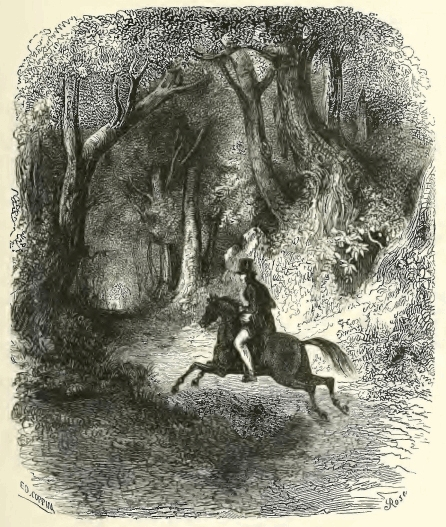
\includegraphics[width=\textwidth]{40254m.jpg}
\end{figure}

“It is probable,” said Albert.

“And since he has sent for me, it is doubtless to question me on what
happened there. What must I answer?”

“The truth.”

“Then I shall say the duel did not take place?”

“You will say I apologized to the Count of Monte Cristo. Go.”

The valet bowed and retired, and Albert returned to his inventory. As
he was finishing this work, the sound of horses prancing in the yard,
and the wheels of a carriage shaking his window, attracted his
attention. He approached the window, and saw his father get into it,
and drive away. The door was scarcely closed when Albert bent his steps
to his mother’s room; and, no one being there to announce him, he
advanced to her bedchamber, and distressed by what he saw and guessed,
stopped for one moment at the door.

As if the same idea had animated these two beings, Mercédès was doing
the same in her apartments that he had just done in his. Everything was
in order,—laces, dresses, jewels, linen, money, all were arranged in
the drawers, and the countess was carefully collecting the keys. Albert
saw all these preparations and understood them, and exclaiming, “My
mother!” he threw his arms around her neck.

The artist who could have depicted the expression of these two
countenances would certainly have made of them a beautiful picture. All
these proofs of an energetic resolution, which Albert did not fear on
his own account, alarmed him for his mother. “What are you doing?”
asked he.

“What were you doing?” replied she.

“Oh, my mother!” exclaimed Albert, so overcome he could scarcely speak;
“it is not the same with you and me—you cannot have made the same
resolution I have, for I have come to warn you that I bid adieu to your
house, and—and to you.”

“I also,” replied Mercédès, “am going, and I acknowledge I had depended
on your accompanying me; have I deceived myself?”

“Mother,” said Albert with firmness. “I cannot make you share the fate
I have planned for myself. I must live henceforth without rank and
fortune, and to begin this hard apprenticeship I must borrow from a
friend the loaf I shall eat until I have earned one. So, my dear
mother, I am going at once to ask Franz to lend me the small sum I
shall require to supply my present wants.”

“You, my poor child, suffer poverty and hunger? Oh, do not say so; it
will break my resolutions.”

“But not mine, mother,” replied Albert. “I am young and strong; I
believe I am courageous, and since yesterday I have learned the power
of will. Alas, my dear mother, some have suffered so much, and yet
live, and have raised a new fortune on the ruin of all the promises of
happiness which heaven had made them—on the fragments of all the hope
which God had given them! I have seen that, mother; I know that from
the gulf in which their enemies have plunged them they have risen with
so much vigor and glory that in their turn they have ruled their former
conquerors, and have punished them. No, mother; from this moment I have
done with the past, and accept nothing from it—not even a name, because
you can understand that your son cannot bear the name of a man who
ought to blush for it before another.”

“Albert, my child,” said Mercédès, “if I had a stronger heart, that is
the counsel I would have given you; your conscience has spoken when my
voice became too weak; listen to its dictates. You had friends, Albert;
break off their acquaintance. But do not despair; you have life before
you, my dear Albert, for you are yet scarcely twenty-two years old; and
as a pure heart like yours wants a spotless name, take my father’s—it
was Herrera. I am sure, my dear Albert, whatever may be your career,
you will soon render that name illustrious. Then, my son, return to the
world still more brilliant because of your former sorrows; and if I am
wrong, still let me cherish these hopes, for I have no future to look
forward to. For me the grave opens when I pass the threshold of this
house.”

“I will fulfil all your wishes, my dear mother,” said the young man.
“Yes, I share your hopes; the anger of Heaven will not pursue us, since
you are pure and I am innocent. But, since our resolution is formed,
let us act promptly. M. de Morcerf went out about half an hour ago; the
opportunity is favorable to avoid an explanation.”

“I am ready, my son,” said Mercédès.

Albert ran to fetch a carriage. He recollected that there was a small
furnished house to let in the Rue des Saints-Pères, where his mother
would find a humble but decent lodging, and thither he intended
conducting the countess. As the carriage stopped at the door, and
Albert was alighting, a man approached and gave him a letter.

Albert recognized the bearer. “From the count,” said Bertuccio. Albert
took the letter, opened, and read it, then looked round for Bertuccio,
but he was gone.

He returned to Mercédès with tears in his eyes and heaving breast, and
without uttering a word he gave her the letter. Mercédès read:

“Albert,—While showing you that I have discovered your plans, I hope
also to convince you of my delicacy. You are free, you leave the
count’s house, and you take your mother to your home; but reflect,
Albert, you owe her more than your poor noble heart can pay her. Keep
the struggle for yourself, bear all the suffering, but spare her the
trial of poverty which must accompany your first efforts; for she
deserves not even the shadow of the misfortune which has this day
fallen on her, and Providence is not willing that the innocent should
suffer for the guilty. I know you are going to leave the Rue du Helder
without taking anything with you. Do not seek to know how I discovered
it; I know it—that is sufficient.

“Now, listen, Albert. Twenty-four years ago I returned, proud and
joyful, to my country. I had a betrothed, Albert, a lovely girl whom I
adored, and I was bringing to my betrothed a hundred and fifty louis,
painfully amassed by ceaseless toil. This money was for her; I destined
it for her, and, knowing the treachery of the sea I buried our treasure
in the little garden of the house my father lived in at Marseilles, on
the Allées de Meilhan. Your mother, Albert, knows that poor house well.
A short time since I passed through Marseilles, and went to see the old
place, which revived so many painful recollections; and in the evening
I took a spade and dug in the corner of the garden where I had
concealed my treasure. The iron box was there—no one had touched
it—under a beautiful fig-tree my father had planted the day I was born,
which overshadowed the spot. Well, Albert, this money, which was
formerly designed to promote the comfort and tranquillity of the woman
I adored, may now, through strange and painful circumstances, be
devoted to the same purpose.

“Oh, feel for me, who could offer millions to that poor woman, but who
return her only the piece of black bread forgotten under my poor roof
since the day I was torn from her I loved. You are a generous man,
Albert, but perhaps you may be blinded by pride or resentment; if you
refuse me, if you ask another for what I have a right to offer you, I
will say it is ungenerous of you to refuse the life of your mother at
the hands of a man whose father was allowed by your father to die in
all the horrors of poverty and despair.”

Albert stood pale and motionless to hear what his mother would decide
after she had finished reading this letter. Mercédès turned her eyes
with an ineffable look towards heaven.

“I accept it,” said she; “he has a right to pay the dowry, which I
shall take with me to some convent!”

Putting the letter in her bosom, she took her son’s arm, and with a
firmer step than she even herself expected she went downstairs.
